% LaTeX-Vorlage zur Erstellung einer Projektarbeit (Dokumentation eines Projekts)
% auf Basis der Vorlage für eine
% Abschlussarbeit in der Fakultät Elektrotechnik, Medien und Informatik an der OTH Amberg-Weiden
% Diese Vorlage entstand im Rahmen des Kurses "LaTeX fürs Studium"
% Aktuelle Version: v0.01
% Stand: 03.06.2023
%
% Changelog:
%
% v0.01: 03.06.2023, Anpassung der Vorlage für Projektarbeiten (article statt report, keine Titelblätter)
%
\documentclass[12pt,oneside]{article}

\usepackage[T1]{fontenc}        % Einstellungen fuer Umlaute usw.
\usepackage[utf8]{inputenc}
\usepackage[ngerman]{babel}
\usepackage{float}              % ermöglicht die Platzierungsoption [H]
\usepackage{enumitem}
\usepackage{graphicx}
\usepackage{subcaption}
\usepackage{xcolor}
\usepackage{parskip}
\usepackage{amsmath}

\usepackage[
    a4paper,                    % Papierformat A4
    left=2.5cm,                 % linker Rand
    right=2.5cm,                % rechter Rand
    top=1.5cm,                  % oberer Rand
    bottom=1.5cm,               % unter Rand
    marginparsep=5mm,           % Abstand der Randnotizen
    marginparwidth=10mm,        % Breite der Randnotizen
    headheight=7mm,             % Hoehe der Kopfzeile
    headsep=1.2cm,              % Abstand der Kopfzeile
    footskip=1.5cm,             % Abstand der Fusszeile
    includeheadfoot
]{geometry}

\usepackage{fancyhdr}                           % Konfiguration von Kopf- und Fusszeilen
\pagestyle{fancy}                               % Seitenstil 'fancy'
\fancyhf{}                                      % vorhandene Einstellungen loeschen
\setlength{\headwidth}{\textwidth}              % Kopf- und Fusszeile so breit wie der Haupttext
\fancyfoot[R]{\thepage}                         % Festlegung des Seitenstils: Seitenzahlen in der Fusszeile rechts
\fancyfoot[L]{\IhreArbeit}                      % Kapitelnr. und -Bezeichnung in der Fusszeile links
\fancyhead[L]{\IhrVornameEins\ \IhrNachnameEins\ \& \IhrVornameZwei\ \IhrNachnameZwei} % Vorname und Name in der Kopfzeile links
\renewcommand{\sectionmark}[1]{                 % Definition der Ausgabe des Kapitels
  \markboth{Abschnitt \thesection. #1}{}}
\renewcommand{\headrulewidth}{0.5pt}            % Trennlinie zwischen Kopfzeile und Haupttext
\renewcommand{\footrulewidth}{0.5pt}            % Trennlinie zwischen Haupttext und Fusszeile
\fancypagestyle{plain}{                         % Anpassung des Seitenstils 'plain' bei Beginn neuer Kapitel
  \fancyhf{}                                    % Vorbelegung loeschen
  \fancyfoot[C]{\thepage}                       % Seitenzeilen in der Fusszeile mittig
}

%\usepackage{amsmath}            % Pakete fuer den Mathematikmodus
%\usepackage{amssymb}
%\usepackage[intlimits]{empheq}

\usepackage[sc]{mathpazo}       % Schriftart Palatino fuer Haupttext und Mathematikmodus
\usepackage{pifont}             % zusaetzliche Symbole

\usepackage[
    format=hang,                % Einstellung fuer Bildunterschriften
    font={footnotesize},
    labelfont={bf},
    margin=1cm,
    aboveskip=5pt,
    position=bottom
]{caption}

\usepackage[svgnames,cmyk,table,hyperref]{xcolor} % Verwendung von Farben

\definecolor{aoenglish}{rgb}{0.0, 0.5, 0.0}
\definecolor{battleshipgrey}{rgb}{0.52, 0.52, 0.51}
\definecolor{cardinal}{rgb}{0.77, 0.12, 0.23}

%\usepackage{tikz}                              % Erstellen von Grafiken
%\usetikzlibrary{positioning,arrows,plotmarks} % TikZ-Bibliotheken
%\usepackage{pgfplots}                          % Darstellung von Plots, Funktionen, Graphen usw.

%
% Weitere Pakete
%
\usepackage{listings}           % Darstellung von Quellcode
\lstloadlanguages{[ISO]C++,Java,XML,[LaTeX]TeX,Python}
\lstset{
    basicstyle=\ttfamily\small,
    keywordstyle=\color{blue},
    commentstyle=\color{green!60!black},
    stringstyle=\color{red},
    breaklines=true,
    showstringspaces=false,
    frame=tb,  % Nur oben und unten Rahmen (sicherer als 'single')
    tabsize=4,
    xleftmargin=0.5cm,
    xrightmargin=0.5cm,
    literate=
    {ö}{{\"o}}1
    {ä}{{\"a}}1
    {ü}{{\"u}}1
    {ß}{{\ss}}1
}

\usepackage[square,numbers,sort]{natbib} % Zitationsstil mit Attribut lastchecked

%
% Persoenliche Angaben
%
\newcommand*{\IhrVornameEins}{Oliver}
\newcommand*{\IhrNachnameEins}{Gaar}
\newcommand*{\IhrVornameZwei}{Bastian}
\newcommand*{\IhrNachnameZwei}{Götz}
\newcommand*{\IhrStudiengang}{Medieninformatik}
\newcommand*{\IhreArbeit}{Computer Vision 1 -- Bonusprojekt \glqq Mai in Amberg\grqq}
\newcommand*{\IhreSchluesselwoerter}{Verkehrsschilder, OpenCV, HSV-Thresholding, Morphologie, Connected Components}
\newcommand*{\IhrErstpruefer}{Prof. Dr. Tatyana Ivanovska}
\newcommand*{\IhrZweitpruefer}{}

\usepackage[
    bookmarks,
    raiselinks,
    pageanchor,
    hyperindex,
    colorlinks,
    citecolor=black,
    linkcolor=black,
    urlcolor=black,
    filecolor=black,
    menucolor=black
]{hyperref}
\hypersetup{
    pdftitle={\IhreArbeit},
    pdfauthor={\IhrVornameEins\ \IhrNachnameEins{} \& \IhrVornameZwei\ \IhrNachnameZwei},
    pdfkeywords={\IhreSchluesselwoerter}
}

%
% Beginn des Textteils
%
\usepackage{cleveref}

\begin{document}
\thispagestyle{empty}

\begin{center}
  \Large
  Ostbayerische Technische Hochschule Amberg-Weiden\\
  Fakultät Elektrotechnik, Medien und Informatik\\[.8cm]
  \IhrErstpruefer\\[.8cm]
  \Large \IhreArbeit\\[.8cm]
  \large \IhrVornameEins\ \IhrNachnameEins\ \&
  \IhrVornameZwei\ \IhrNachnameZwei\\[.8cm]
  \large Studiengang \IhrStudiengang\\[.8cm]
  \today\\[2.0cm]
\end{center}

\tableofcontents
\clearpage

\section{Einleitung und Aufgabenstellung}

Im Rahmen des Projekts werden Verkehrsschilder in Amberg segmentiert. Ziel hierbei ist es, Schilder mit Bounding Boxes zu segmentieren und diese einer Klasse zuzuordnen.

Dabei werden nur Methoden verwendet, die im Rahmen der Vorlesung behandelt wurden.

Verwendete Verfahren sind HSV-Thresholding, mathematische Morphologie und Connected Components.

Entsprechend der Vorlesung wurde folgendermaßen vorgegangen:

\begin{center}
\textbf{Prepare Data $\rightarrow$ Preprocessing $\rightarrow$ Processing $\rightarrow$ Postprocessing $\rightarrow$ Evaluation}
\end{center}

Die folgenden Abschnitte beschreiben und begründen die entsprechend gewählten Methoden mit Verweis auf die zugehörige Vorlesung, diskutieren verworfene Ansätze und evaluieren zum Schluss unsere Ergebnisse.

\section{Bilder}

Die Bilder wurden im Stadtgebiet Amberg bei gutem Wetter und Tageslicht aufgenommen. Insgesamt entstanden mehr als 20 Bilder. In der Auswertung werden gemäß Projektvorgabe maximal 20 Bilder verwendet. Die Originalauflösung der Fotos beträgt $3024 \times 4032$ Pixel.

Die Schilder wurden manuell nach ihrem Verkehrsschild-Typ gelabelt (siehe Klassenschema in Abschnitt~\ref{sec:klassifikation}). Als Referenzwert dient pro Bild die Anzahl der tatsächlich vorhandenen Schilder je Klasse. Eine Bounding-Box-Annotation wurde nicht erstellt. Die Auffangklasse \glqq Unbekannt\grqq{} kommt im Referenzwert nicht vor, sie entsteht nur innerhalb der Pipeline, wenn eine Detektion keiner definierten Regel zugeordnet werden kann.

\begin{figure}[H]
  \centering
  \begin{subfigure}{0.32\textwidth}
    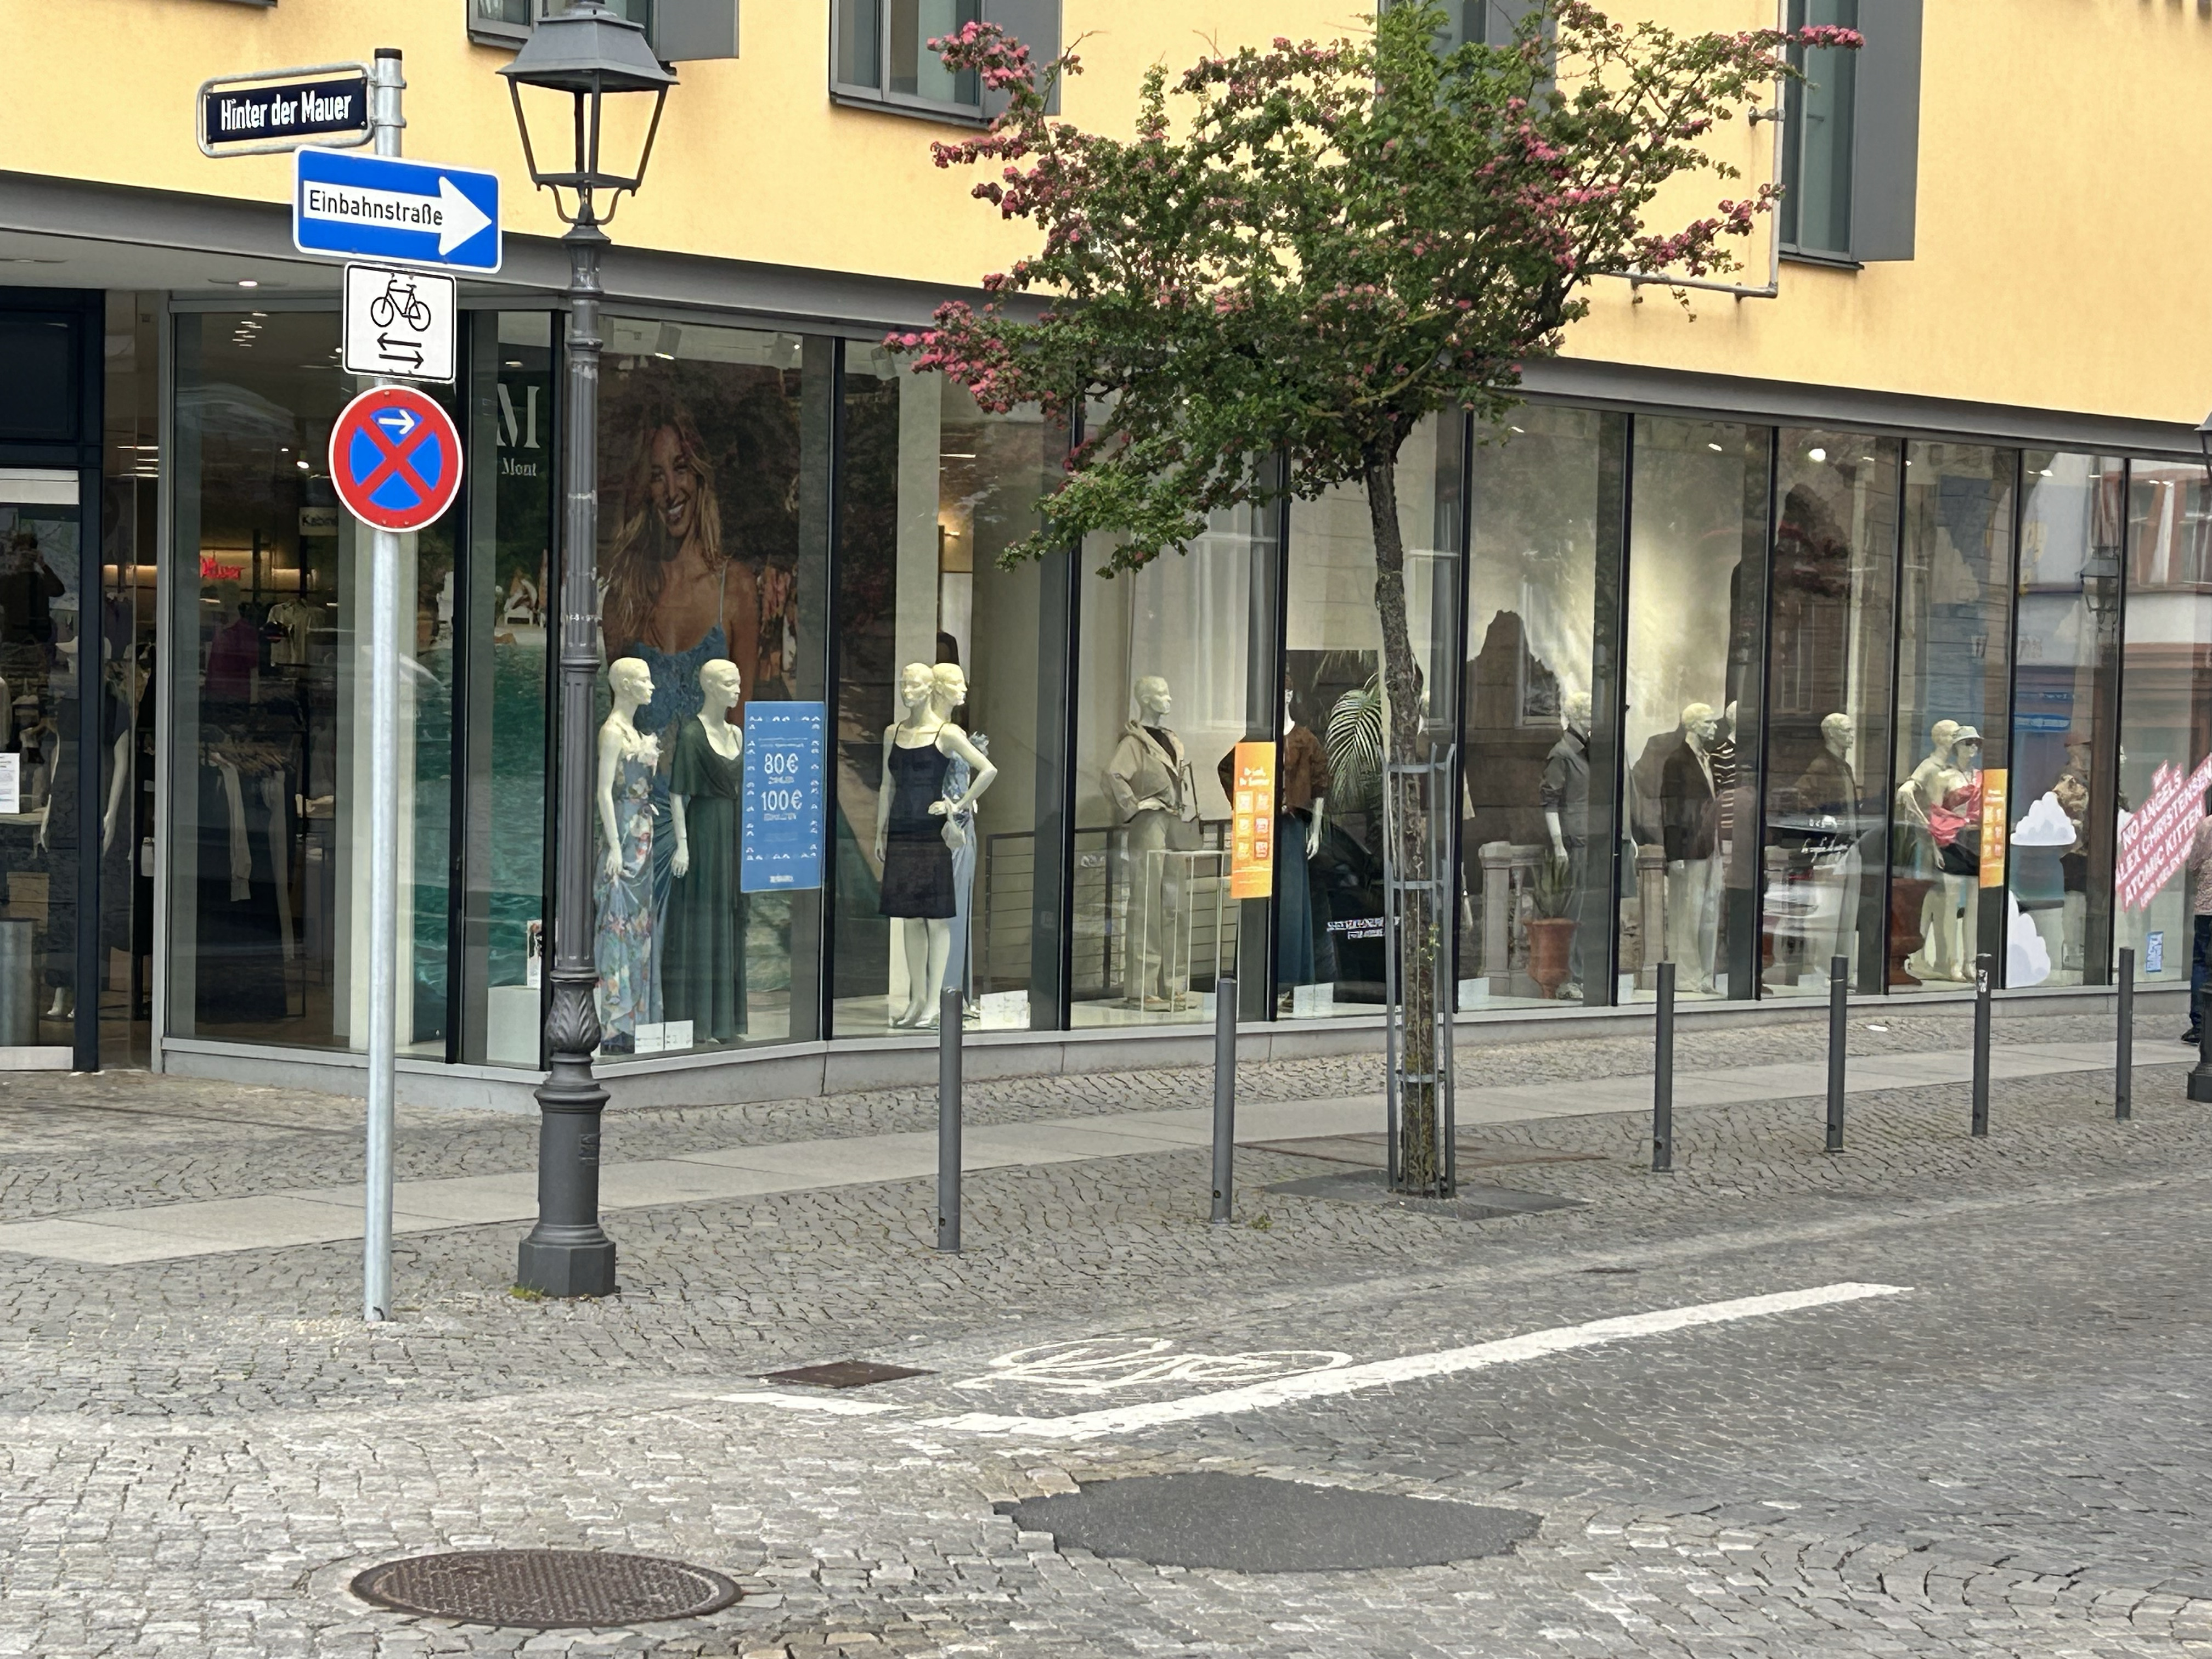
\includegraphics[width=\textwidth]{images/IMG_2429.jpeg}
    \caption{Beispielbild 1}
  \end{subfigure}
  \hfill
  \begin{subfigure}{0.32\textwidth}
    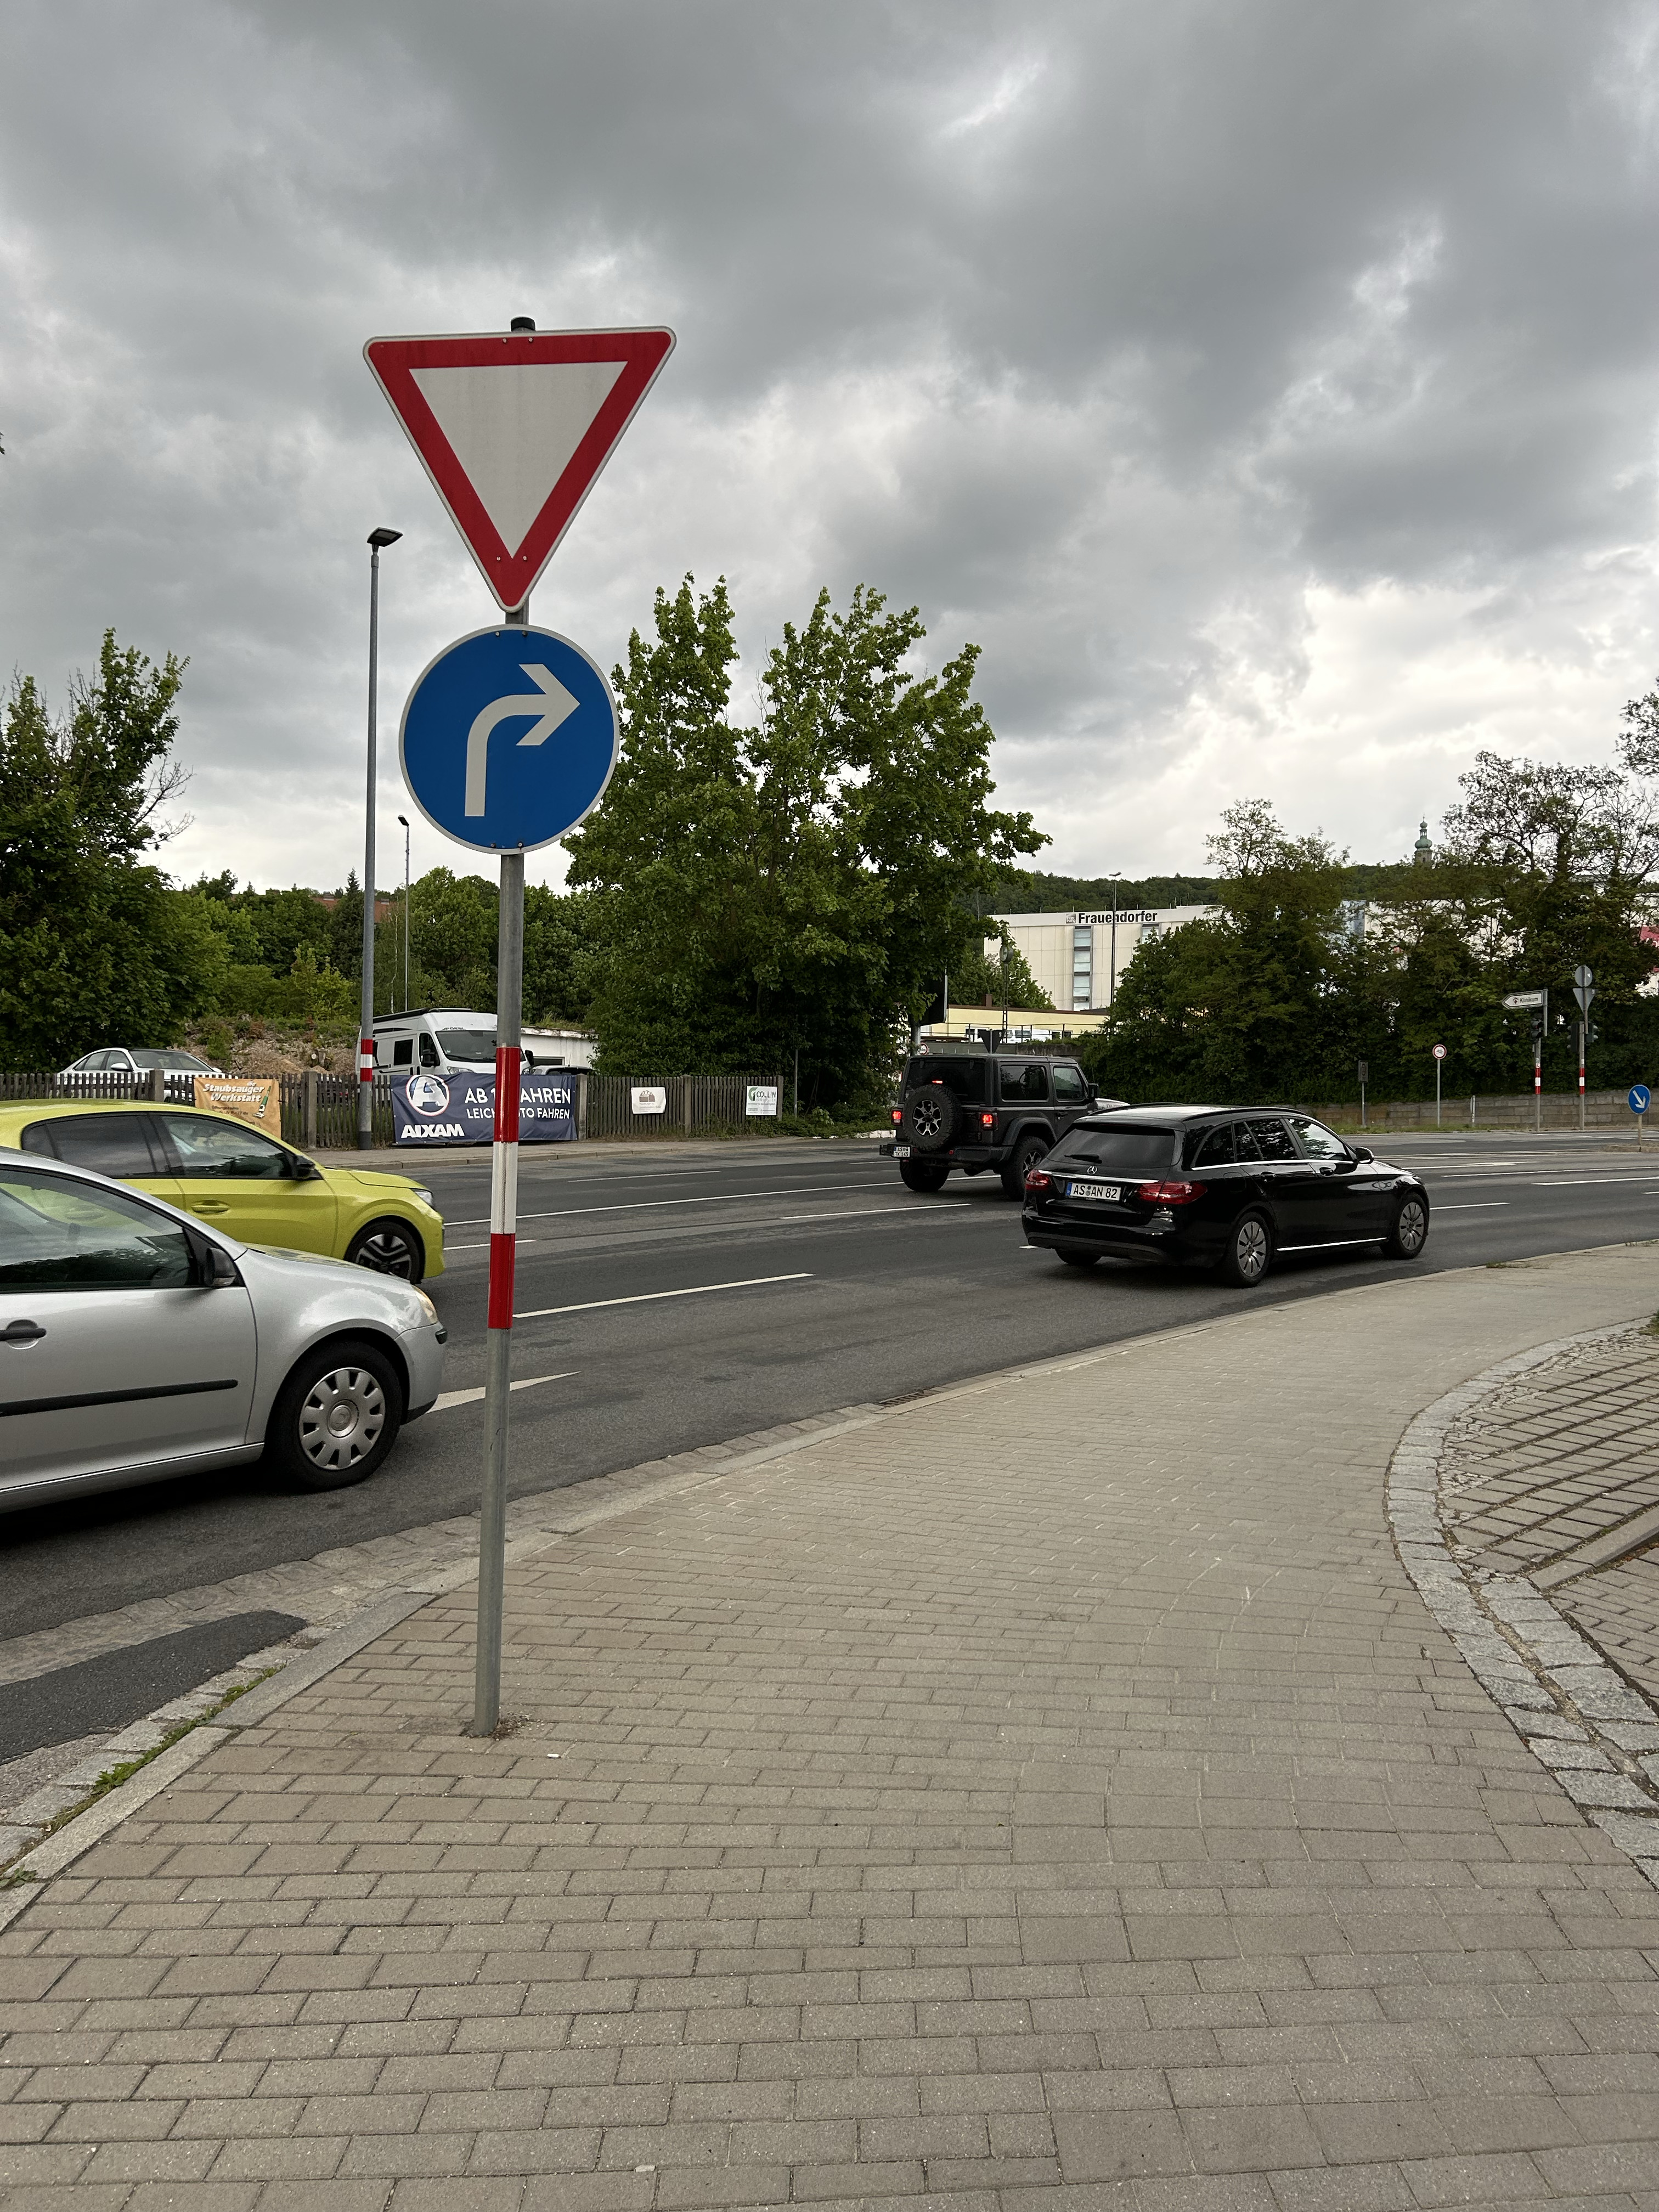
\includegraphics[width=\textwidth]{images/IMG_2521.jpeg}
    \caption{Beispielbild 2}
  \end{subfigure}
  \hfill
  \begin{subfigure}{0.32\textwidth}
    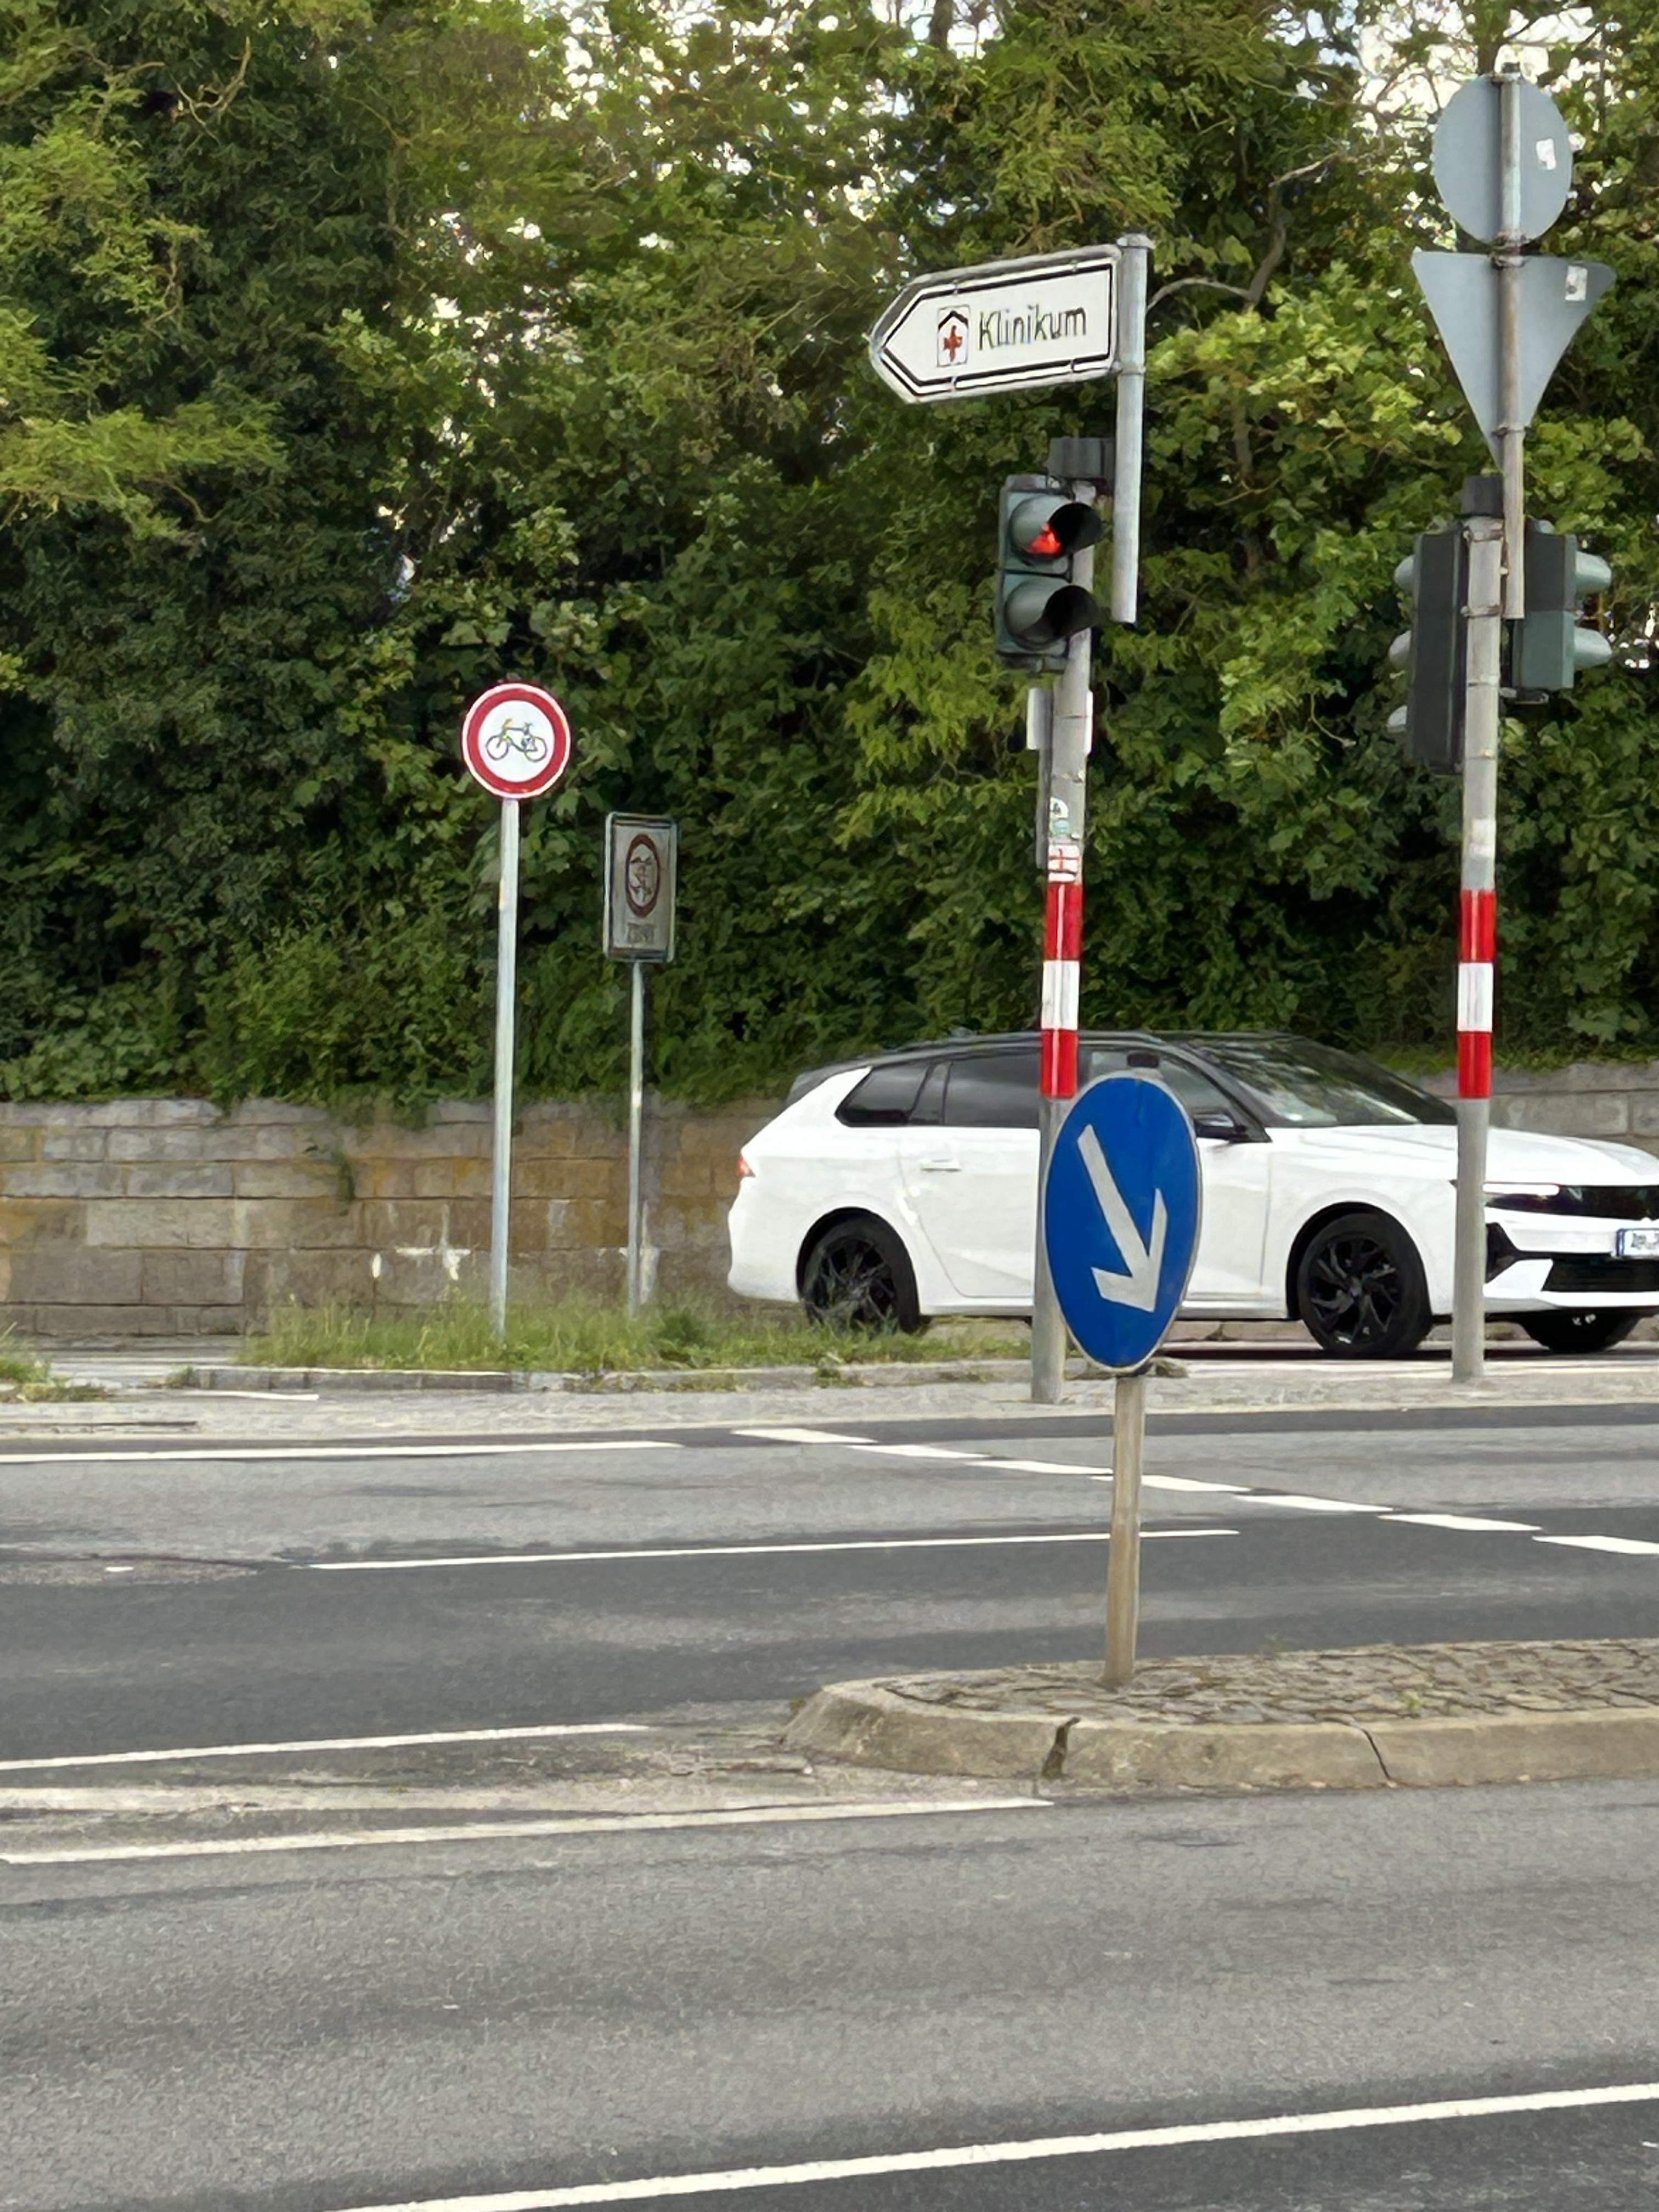
\includegraphics[width=\textwidth]{images/IMG_2522.jpeg}
    \caption{Beispielbild 3}
  \end{subfigure}
  \caption{Repräsentative Beispielbilder aus Amberg.}
\end{figure}

\section{Preprocessing}

\subsection{Skalierung}

Die Bilder werden unter Beibehaltung des Seitenverhältnisses auf eine Breite von 800 Pixel herunterskaliert. Die hohe Originalauflösung verlangsamt viele Verarbeitungsschritte unnötig, und eine einheitliche Bildgröße ermöglicht eine konsistente Parameterwahl über alle Bilder hinweg.

\subsection{Entrauschen -- Bilateral Filter (VL 4)}

Zur Rauschreduktion wird ein Bilateral-Filter eingesetzt (Parameter: $d = 9$, sigmaColor $= 75$, sigmaSpace $= 75$). Vorlesung 4 stellt mehrere Entrauschungsverfahren vor. Diese wurden in einem Vorversuch verglichen:

\begin{table}[H]
\centering
\begin{tabular}{|l|l|l|l|}
\hline
\textbf{Methode} & \textbf{Kantenerhalt} & \textbf{Geschwindigkeit} & \textbf{Bewertung} \\
\hline
Gaussian Filter & gering (Kanten verwischt) & schnell & ungeeignet \\
\textbf{Bilateral Filter} & hoch & gut & \textbf{gewählt} \\
Anisotropic Diffusion & hoch & langsam & verworfen \\
Non-Local Means & sehr hoch & sehr langsam & verworfen \\
\hline
\end{tabular}
\caption{Vergleich der Entrauschungsverfahren aus Vorlesung 4.}
\end{table}

Der Bilateral-Filter wurde gewählt, weil er Kanten zuverlässig erhält -- entscheidend für die Beibehaltung der klaren Schildkonturen -- und dabei eine gute Laufzeit bietet. Anisotropic Diffusion und Non-Local Means lieferten kaum bessere Ergebnisse bei deutlich höherem Rechenaufwand.

\subsection{Farbraumwechsel RGB nach HSV (VL 6)}

Das \glqq entrauschte\grqq{} Bild wird in den HSV-Farbraum konvertiert. Der HSV-Raum ist praktisch, da man in diesem leicht bestimmte Farben filtern kann. Dies wurde sich zunutze gemacht, da Verkehrsschilder grundsätzlich mit Signalfarben gekennzeichnet sind. Dadurch kann man diese relativ gut mit einem HSV-Thresholding segmentieren.

\section{Processing -- Farbsegmentierung im HSV-Raum (VL 6)}

Die eigentliche Segmentierung erfolgt durch HSV-basiertes Thresholding (\texttt{cv2.inRange}). Für die drei relevanten Schildfarben Rot, Blau und Gelb wird je eine Maske erzeugt:

\begin{table}[H]
\centering
\begin{tabular}{|l|l|l|l|}
\hline
\textbf{Farbe} & \textbf{H-Bereich} & \textbf{S-Bereich} & \textbf{V-Bereich} \\
\hline
Rot  & 0--10$^\circ$ und 170--179$^\circ$ & 125--255 & 50--250 \\
Blau & 90--120$^\circ$ & 80--255 & 50--255 \\
Gelb & 18--27$^\circ$ & 130--220 & 100--200 \\
\hline
\end{tabular}
\caption{Verwendete HSV-Schwellwertbereiche je Farbe.}
\end{table}

Rot liegt im HSV-Farbraum am Übergang des Farbkreises und wird daher über zwei Teilbereiche definiert, die per ODER kombiniert werden.

\begin{figure}[H]
  \centering
  \begin{subfigure}{0.24\textwidth}
    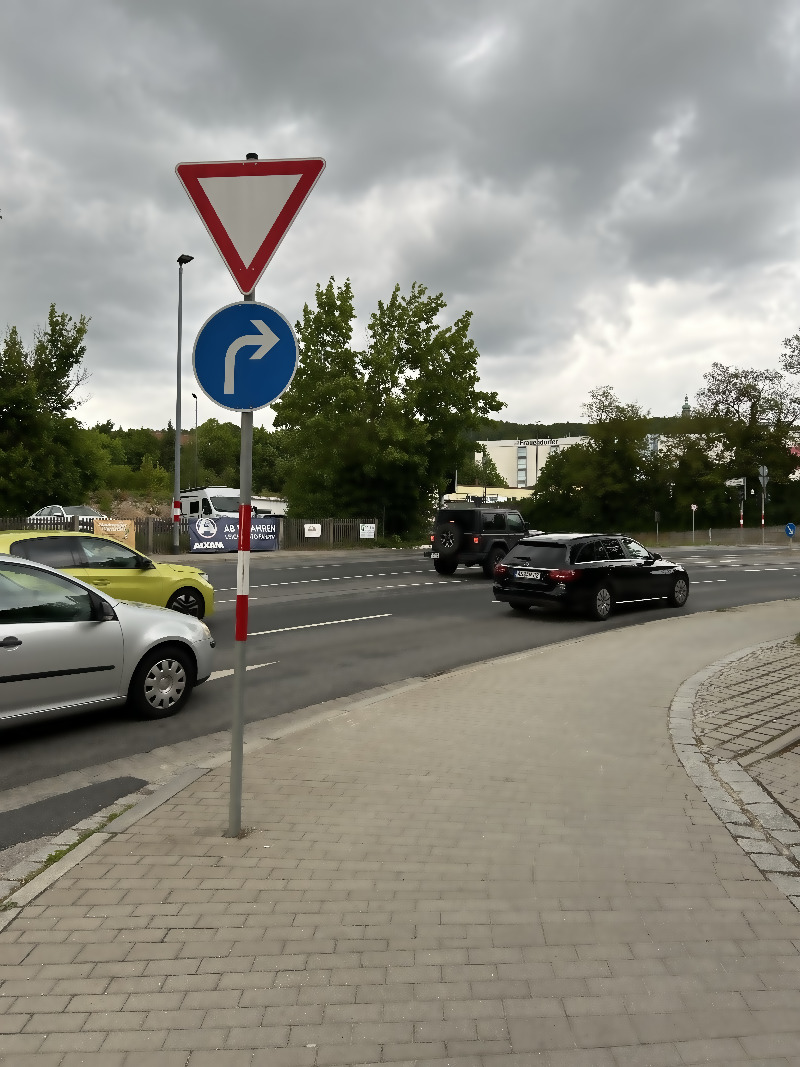
\includegraphics[width=\textwidth]{images/IMG_2521/bilateral_filter.jpeg}
    \caption{Orignal nach Bilateral-Filter}
  \end{subfigure}
  \hfill
  \begin{subfigure}{0.24\textwidth}
    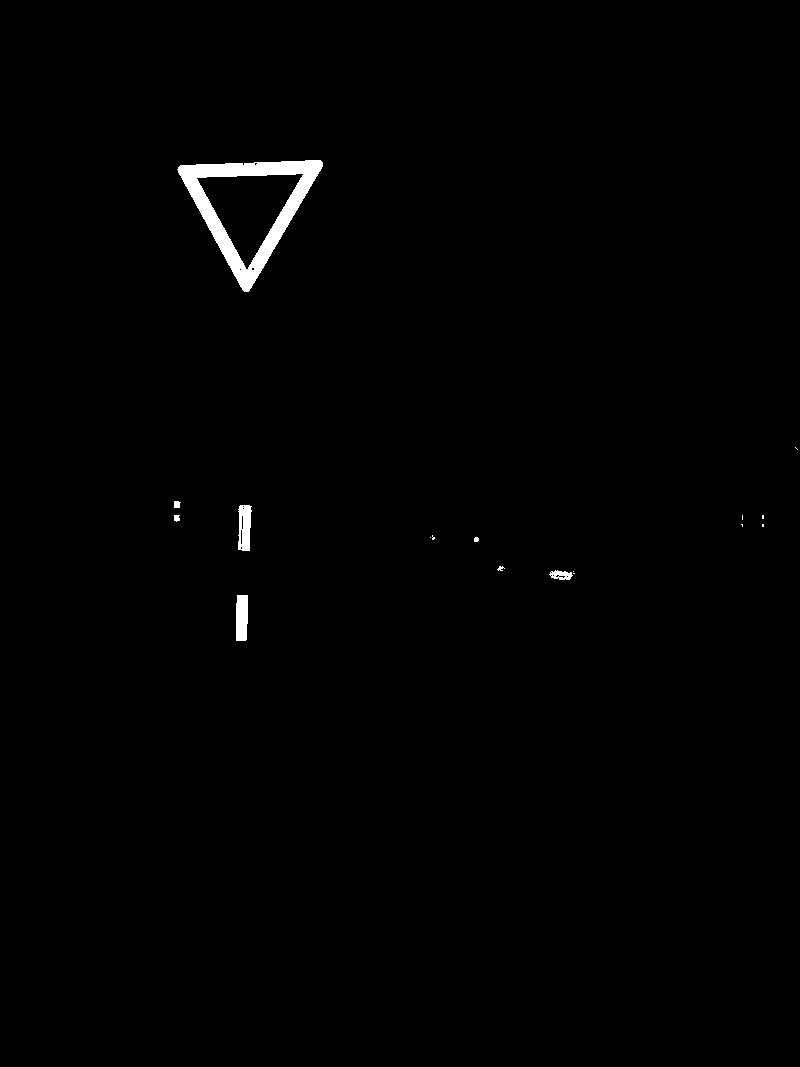
\includegraphics[width=\textwidth]{images/IMG_2521/maske_rot.jpeg}
    \caption{Binäre Maske für Rot}
  \end{subfigure}
  \hfill
  \begin{subfigure}{0.24\textwidth}
    
\includegraphics[width=\textwidth]{images/IMG_2521/maske_blau.jpeg}
    \caption{Binäre Maske für Blau}
  \end{subfigure}
  \hfill
  \begin{subfigure}{0.24\textwidth}
    
\includegraphics[width=\textwidth]{images/IMG_2521/maske_gelb.jpeg}
    \caption{Binäre Maske für Gelb}
  \end{subfigure}
  \caption{Binäre Farbmasken vor der morphologischen Bereinigung}
\end{figure}

\section{Postprocessing}

\subsection{Morphologische Bereinigung (VL 5)}

Die rohen Masken enthalten noch kleine Rauschartefakte und Löcher. Sie werden mit mathematischer Morphologie bereinigt:

\begin{itemize}
\item \textbf{Opening} (Erosion gefolgt von Dilatation), elliptisches Strukturelement $4 \times 4$, 1 Iteration: entfernt kleine Pixelfragmente.
\item \textbf{Closing} (Dilatation gefolgt von Erosion), elliptisches Strukturelement $7 \times 7$, 2 Iterationen: schließt Lücken innerhalb der Schildfläche.
\end{itemize}

\begin{figure}[H]
    \centering
    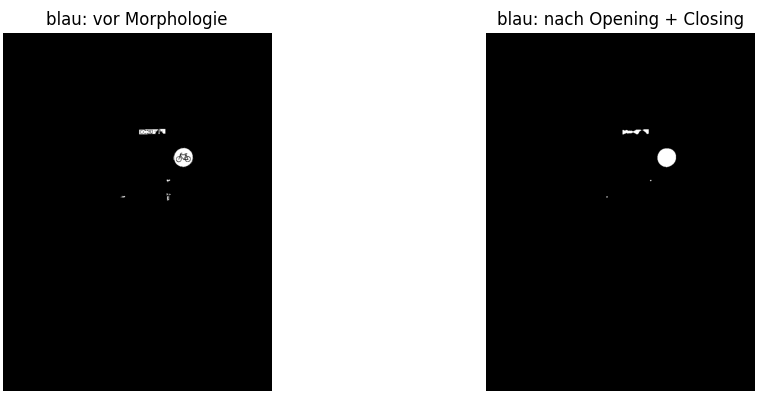
\includegraphics[width=0.8\textwidth]{images/ergebnisse/Morphologie_Beispiel.png}
    \caption{Maske vor und nach Morphologischer Bereinigung}
    \label{fig:meinbild}
\end{figure}

\subsection{Connected-Component-Analyse (VL 5)}

Auf jeder bereinigten Maske werden mit \texttt{cv2.connectedComponentsWithStats} die zusammenhängenden Regionen bestimmt. Verwendet wird die 8er-Nachbarschaft (N8 aus Vorlesung 1). Jede Komponente wird anhand folgender Kriterien gefiltert:

\begin{itemize}
\item Mindestfläche MIN\_AREA $= 600$\,px: beachtet kleine Artefakte nicht.
\item Aspect Ratio $0{,}5 \leq w/h \leq 2{,}0$ -- schließt sehr schmale oder breite Formen aus.
\end{itemize}

Für jede gültige Komponente werden Bounding Box, Fläche, Schwerpunkt und Aspect Ratio gespeichert.

\subsection{Bounding Box innerhalb einer Bounding Box entfernen}

Abschließend werden die gefundenen Schilder absteigend nach Fläche sortiert. Kleinere Bounding Boxes, die vollständig innerhalb einer größeren liegen, werden entfernt. So werden sinnlose Artefakte entfernt und beispielsweise im Falle eines Park-/Halteverbotsschildes die innere Fläche nicht zusätzlich segmentiert.

\begin{figure}[H]
  \centering
  \begin{subfigure}{0.32\textwidth}
    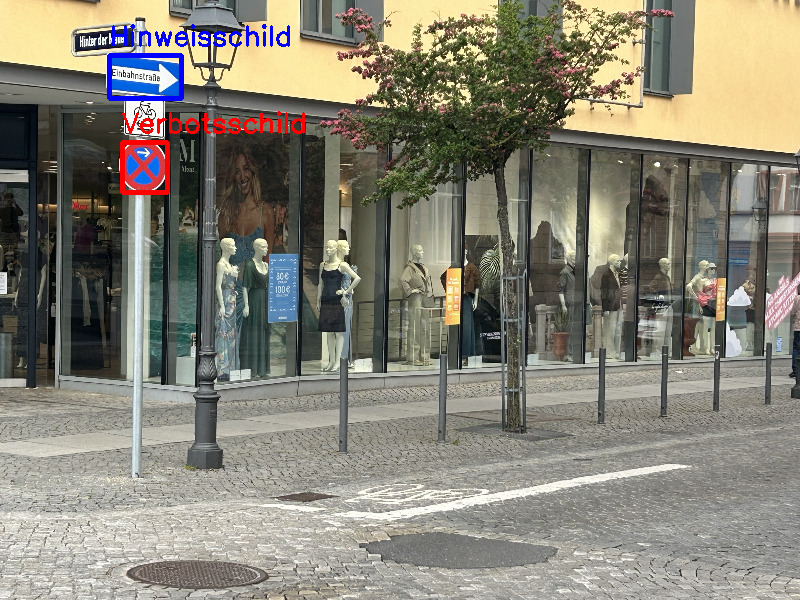
\includegraphics[width=\textwidth]{images/ergebnisse/ergebnis_IMG_2429.jpeg}
  \end{subfigure}
  \hfill
  \begin{subfigure}{0.32\textwidth}
    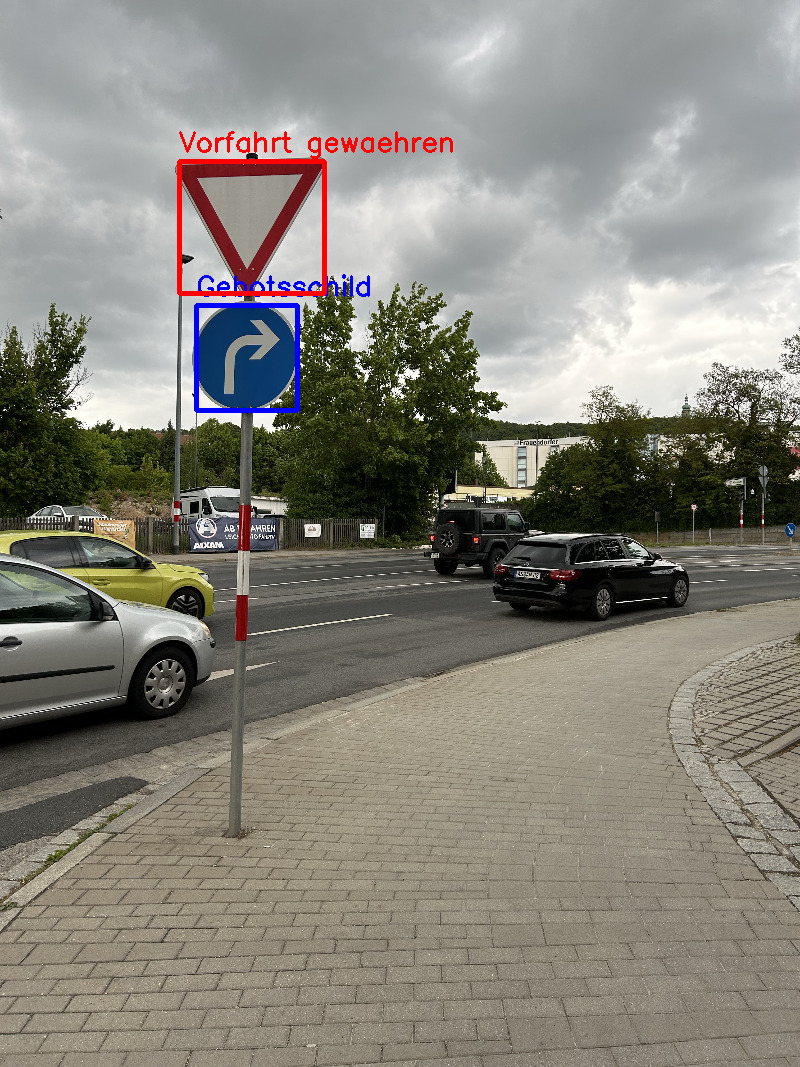
\includegraphics[width=\textwidth]{images/ergebnisse/ergebnis_IMG_2521.jpeg}
  \end{subfigure}
  \hfill
  \begin{subfigure}{0.32\textwidth}
    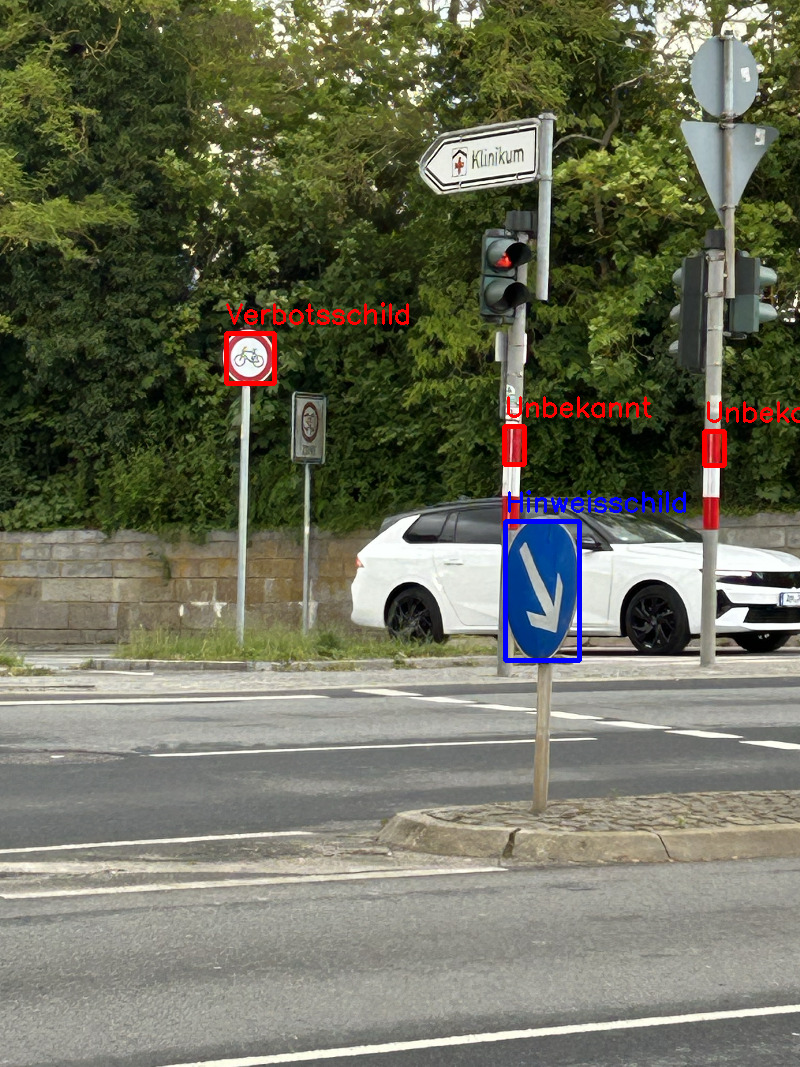
\includegraphics[width=\textwidth]{images/ergebnisse/ergebnis_IMG_2522.jpeg}
  \end{subfigure}
  \hfill
  \caption{Endergebnisse der Pipline}
\end{figure}

\section{Klassifikation}
\label{sec:klassifikation}

Die Zuordnung zur Schildklasse erfolgt regelbasiert anhand von Farbe und Geometrie. Als Geometriemerkmale dienen der Füllgrad (Verhältnis von Objektfläche zur Bounding-Box-Fläche, area/bbox) sowie das Seitenverhältnis $w/h$ und der geometrische Schwerpunkt. Dabei wurde für die Evaluation Warnung\_Vorfahrt und Warnung\_Vorfahrt (Vorfahrtss.) vereinigt. Die Unterscheidung dient nur für die Textlabels der Bounding Boxen in den Bildern.
Die Klassifizierungsregeln sind:

\begin{table}[H]
\centering
\begin{tabular}{|c|l|l|l|}
\hline
\textbf{\#} & \textbf{Farbe} & \textbf{Form-Bedingung} & \textbf{Klasse} \\
\hline
1 & Rot  & $0{,}75 \leq w/h \leq 1{,}25$ und area/bbox $> 0{,}30$ & Verbot\_Stop  \\
2 & Rot  & $0{,}75 \leq w/h \leq 1{,}25$, area/bbox $\leq 0{,}30$, $\text{cyrel} > 0{,}55$ & Warnung\_Vorfahrt \\
3 & Rot  & $0{,}75 \leq w/h \leq 1{,}25$, area/bbox $\leq 0{,}30$,  $\text{cyrel} < 0{,}45$ & Warnung\_Vorfahrt (Vorfahrtss.) \\
4 & Blau & $0{,}75 \leq w/h \leq 1{,}25$ & Gebot \\
5 & Blau & $w/h < 0{,}75$ oder $w/h > 1{,}25$ & Hinweis \\
6 & Gelb & $0{,}85 \leq w/h \leq 1{,}20$ & Vorfahrtsstrasse \\
7 & Gelb & $w/h < 0{,}80$ & Ortstafel\_Wegweiser \\
8 & --   & trifft auf keine Regel zu & Unbekannt \\
\hline
\end{tabular}
\caption{Klassifikationsregeln.}
\end{table}

\section{Verworfene Ansätze und Erkenntnisse}

Im Folgenden wird auf Methoden eingegangen, die getestet, aber nicht in die finale Pipeline übernommen wurden.

\subsection{Beleuchtungskorrektur: Histogram Equalization und CLAHE (VL 6)}

Zur Kompensation von Unter-/ Überbelichtung wurden Histogram Equalization sowie CLAHE auf dem V-Kanal des HSV Bildes getestet. In der Praxis zeigte sich jedoch nahezu kein Unterschied für das nachgelagerte HSV-Thresholding. Da die Segmentierung hauptsächlich über Farbton (H) und Sättigung (S) erfolgt und die V-Schwellen ohnehin großzügig gewählt sind, brachte die Helligkeitsanpassung keinen ersichtlichen Mehrwert. Die Beleuchtungskorrektur wurde deswegen weggelassen, um die Pipeline schlank zu halten.

\subsection{Otsu-Thresholding für Zusatzschilder (VL 7)}

Es wurde versucht, die weißen Zusatzschilder die oft unter einem Schild stehen zu segmentieren. Hierfür wurde nur der Bereich unter einem bereits segmentierten Schild \glqq ausgeschnitten\grqq{} und versucht, mit einem Otsu-Thresholding die kleinen rechteckigen Zusatzschilder zu erkennen. Da diese sich nicht zuverlässig vom Hintergrund trennen ließen, lieferte es keine stabilen Ergebnisse. Dieser Ansatz wurde daher verworfen.

\section{Evaluation}

Die Evaluation erfolgt auf Zählebene. Für jedes Bild wird geprüft, ob die Pipeline die korrekte Anzahl an Schildern je Klasse erkennt. Abweichungen treten als nicht erkannte Schilder (False Negatives) oder als falsch klassifizierte Schilder (False Positives) auf.

Es könnte auch vorkommen, dass ein Objekt im Vordergrund fälschlicherweise als Schild einer Klasse erkannt wird, das eigentliche Schild jedoch nicht. Solche Fälle müsste man manuell prüfen.

Die Pipeline wurde auf 20 Bildern mit insgesamt 55 vorhandenen Schildern ausgewertet.

Die daraus resultierenden Ergebnisse sind in der folgenden Tabelle zusammengefasst:

\begin{table}[H]
\centering
\begin{tabular}{|l|c|c|c|c|c|c|}
\hline
\textbf{Klasse} & \textbf{TP} & \textbf{FP} & \textbf{FN} & \textbf{Precision} & \textbf{Recall} & \textbf{F1} \\
\hline
Verbot / Stop                  & 8 & 1  & 15 & 0{,}89 & 0{,}35 & 0{,}50 \\
Warnung / Vorfahrt gewähren    & 4 & 0  & 2  & 1{,}00 & 0{,}67 & 0{,}80 \\
Gebot                          & 4 & 6  & 7  & 0{,}40 & 0{,}36 & 0{,}38 \\
Hinweis                        & 6 & 4  & 5  & 0{,}60 & 0{,}55 & 0{,}57 \\
Vorfahrtsstraße                & 1 & 1  & 1  & 0{,}50 & 0{,}50 & 0{,}50 \\
Ortstafel / Wegweiser          & 0 & 0  & 2  & --     & -- & -- \\
\hline
\end{tabular}
\caption{Auswertungsergebnisse auf 20 Bildern}
\end{table}

\textbf{Gesamtbild.}  Die F1-Werte je Klasse liegen zwischen 0,00 (Ortstafel/Wegweiser) und 0,80 (Warnung/Vorfahrt gewähren) und schwanken damit erheblich. Auffällig ist über fast alle Klassen hinweg ein deutliches Ungleichgewicht zwischen Precision und Recall. Wenn ein Schild erkannt wird, ist die Klassifikation oft korrekt (Precision bei drei von sechs Klassen größer gleich 0,6), aber von 55 echten Schildern werden insgesamt 32 übersehen. Die Hauptschwäche ist damit eindeutig die Sensitivität, nicht die Genauigkeit.

\textbf{Was die Daten bestätigen.} Verbot/Stop hat mit 15 False Negatives die mit Abstand meisten übersehenen Schilder, gleichzeitig aber eine sehr hohe Precision von 0,89. Der Grund hierfür ist,dass in vielen von den genutzten Bildern sich Verbot/Stop-Schilder im Hintergrund befinden und somit die Pixelfläche zu klein ist. Diese fallen durch entweder durch den MIN\_AREA-Filter oder gehen zuvor beim Opening/ Closing verloren. Die roten Schilder, die groß genug sind, werden zuverlässig erkannt. Ortstafel/Wegweiser verfehlt die Pipeline hier vollständig (0 TP bei 2 echten Schildern). Beim Betrachten der Pipeline-Ausgaben zeigt sich, dass zumindest eines dieser Schilder zwar detektiert, jedoch als „Unbekannt" klassifiziert wurde. Dies verdeutlicht, dass die Klassifikation noch nicht genau genug arbeitet. Erschwert wird eine eindeutige Zuordnung zusätzlich durch die stark variierenden Größen dieser Schilder in der Realität.

\textbf{Klassenspezifische Beobachtungen.} Die schwächste Klasse ist Gebot (F1 $= 0{,}38$) mit zugleich vielen False Positives (6) und False Negatives (7). Da Gebot und Hinweis sich nur über das Seitenverhältnis unterscheiden ($w/h \approx 1$ vs. $w/h \neq 1$), führt diese harte Schwelle bei blauen Objekten, die nahezu quadratisch sind, zu wechselseitigen Fehlzuordnungen.Hinweisschilder werden als Gebot klassifiziert und umgekehrt. Bei Warnung/Vorfahrt gewähren ist die Precision dagegen perfekt (1,00) bei einem Recall von 0,67: Alle erkannten Schilder sind korrekt klassifiziert, ein Teil der tatsächlich vorhandenen wird jedoch nicht erfasst.

\textbf{Einordnung.} Mit 20 Bildern und Klassengrößen von teilweise nur zwei echten Schildern (Vorfahrtsstraße, Ortstafel/Wegweiser) sind die Klasse-Metriken statistisch wenig aussagekräftig. Einzelne Fehler schlagen voll auf Precision und Recall durch. Für eine fundierte Aussage über die Pipeline-Qualität wäre eine deutlich größere und ausgewogenere Bildmenge erforderlich.

\section{Bekannte Grenzen und Ausblick}
\label{sec:grenzen}

\begin{itemize}
\item Die Evaluation erfolgt zählbasiert ohne Lokalisierungsmaß, da keine Bounding-Box-Annotation vorliegt.

\item Weiter entfernte Schilder umfassen aufgrund ihrer geringen Pixelanzahl zu wenige Bildpunkte und werden daher vom \texttt{MIN\_AREA}-Filter herausgefiltert, sodass Schilder im Hintergrund nicht mehr segmentiert werden. Der Filter wurde eingeführt, um störende Artefakte in der Segmentierung zu reduzieren. Dies geht jedoch zulasten der Erkennung weiter entfernter Schilder. Während die Anzahl unerwünschter Artefakte sinkt, werden Schilder im Hintergrund nicht mehr zuverlässig erfasst.

\item Objekte, die in einem gleichen oder ähnlichen Farbbereich wie die Schilder liegen, können fälschlicherweise mitsegmentiert und anschließend gegebenenfalls auch fälschlicherweise als Schilder klassifiziert werden. Durch eine präzise Abstimmung der Farbbereiche sowie den Einsatz des \texttt{MIN\_AREA}-Filters und morphologischer Operationen wurde versucht, diesen Effekt so weit wie möglich einzudämmen. Dennoch treten bei größeren zusammenhängenden Flächen mit ähnlicher Farbgebung weiterhin vereinzelt unerwünschte Artefakte auf.

\item Zusatzschilder die oft unter Verkehrszeichen zu finden sind, konnten wir nicht sinnvoll segmentieren, weshalb dies entfiel.
\item Die Klassifizierung hat ihre Grenzen, weshalb die Schilder in 7 definierte Klassen eingeteilt wurden. Es kann beispielsweise nicht erkannt werden, welche Geschwindigkeit gefahren werden muss, geschweige denn, dass das Temposchild nicht als solches klassifiziert werden kann, sondern direkt als ein Verbotsschild klassifiziert wird.
\item Um die Generalisierung optimal zu testen, sollte man mehr als 20 Bilder nutzen. Zudem hätte man Bilder durch Rauschen variieren können, um zu prüfen, ob die Pipeline standhaft bleibt. Es hätte dementsprechend sinnvoll sein können, Bilder nicht nur bei gutem Wetter an einem Tag, sondern über mehrere Tage auch bei schlechtem Wetter zu machen.
\end{itemize}

Insgesamt zeigt sich jedoch, dass eine konsequent klassische Pipeline aus HSV-Thresholding, Morphologie und Connected Components für die farbbasierte Erkennung von Verkehrsschildern ein tragfähiger Ansatz ist.

\appendix
\section{GitHub repository}
Der im Rahmen dieser Arbeit entwickelte Quellcode ist unter folgendem Repository verfügbar: \url{https://github.com/CycleByte/CV_Projekt_SS2026}.
\end{document}

